\section{Results}
\label{sec:results}

We present detection scores across conditions (\secref{sec:main_results}), the per-round trajectory of iterative rejection (\secref{sec:trajectory}), the comparison with best-of-5 selection (\secref{sec:bon}), and linguistic feature analysis (\secref{sec:linguistic}).

\subsection{Main Detection Results}
\label{sec:main_results}

\tabref{tab:binoculars_results} and \tabref{tab:roberta_results} show mean detection scores across all conditions for both detectors.

\begin{table}[t]
\centering
\caption{Detection scores by condition (\binoculars, zero-shot). Lower $P(\text{AI})$ indicates more successful evasion. Best AI-generated result in \textbf{bold}. Human text shown for calibration.}
\label{tab:binoculars_results}
\begin{tabular}{@{}lccc@{}}
\toprule
\textbf{Condition} & \textbf{Mean $P(\text{AI})$} & \textbf{Std} & \textbf{$\Delta$ vs.\ Vanilla} \\
\midrule
Human text & 0.325 & 0.376 & --- \\
\midrule
Vanilla & 0.798 & 0.236 & baseline \\
Single-step & 0.835 & 0.228 & $+$0.037 \\
\textbf{Strong single-step} & \textbf{0.342} & 0.292 & $-$\textbf{0.456} \\
Iterative (R5) & 0.483 & 0.280 & $-$0.315 \\
Best-of-5 (selected) & 0.702 & 0.286 & $-$0.096 \\
\bottomrule
\end{tabular}
\end{table}

\begin{table}[t]
\centering
\caption{Detection scores by condition (\roberta, trained classifier). This detector assigns human text a \emph{higher} AI probability (0.320) than vanilla \gptfour (0.264), indicating poor generalization to modern LLM outputs. Results included for completeness but should be interpreted with caution.}
\label{tab:roberta_results}
\begin{tabular}{@{}lccc@{}}
\toprule
\textbf{Condition} & \textbf{Mean $P(\text{AI})$} & \textbf{Std} & \textbf{$\Delta$ vs.\ Vanilla} \\
\midrule
Human text & 0.320 & 0.334 & --- \\
\midrule
Vanilla & 0.264 & 0.387 & baseline \\
Single-step & 0.294 & 0.400 & $+$0.030 \\
\textbf{Strong single-step} & \textbf{0.039} & 0.147 & $-$\textbf{0.225} \\
Iterative (R5) & 0.082 & 0.226 & $-$0.182 \\
Best-of-5 (selected) & 0.103 & 0.257 & $-$0.161 \\
\bottomrule
\end{tabular}
\end{table}

Three findings stand out. First, iterative rejection substantially reduces detection: from 0.798 to 0.483 on \binoculars ($-$39.5\%). Second, the strong single-step prompt achieves an even larger reduction to 0.342 ($-$57.1\%), approaching human text levels. Third, the naive single-step prompt (\ie ``write naturally'') is counterproductive, slightly \emph{increasing} detection scores on \binoculars (0.835 vs.\ 0.798).

\Figref{fig:condition_comparison} shows the distribution of scores across conditions, illustrating that the strong single-step and iterative rejection conditions shift the score distribution substantially leftward.

\begin{figure}[t]
\centering
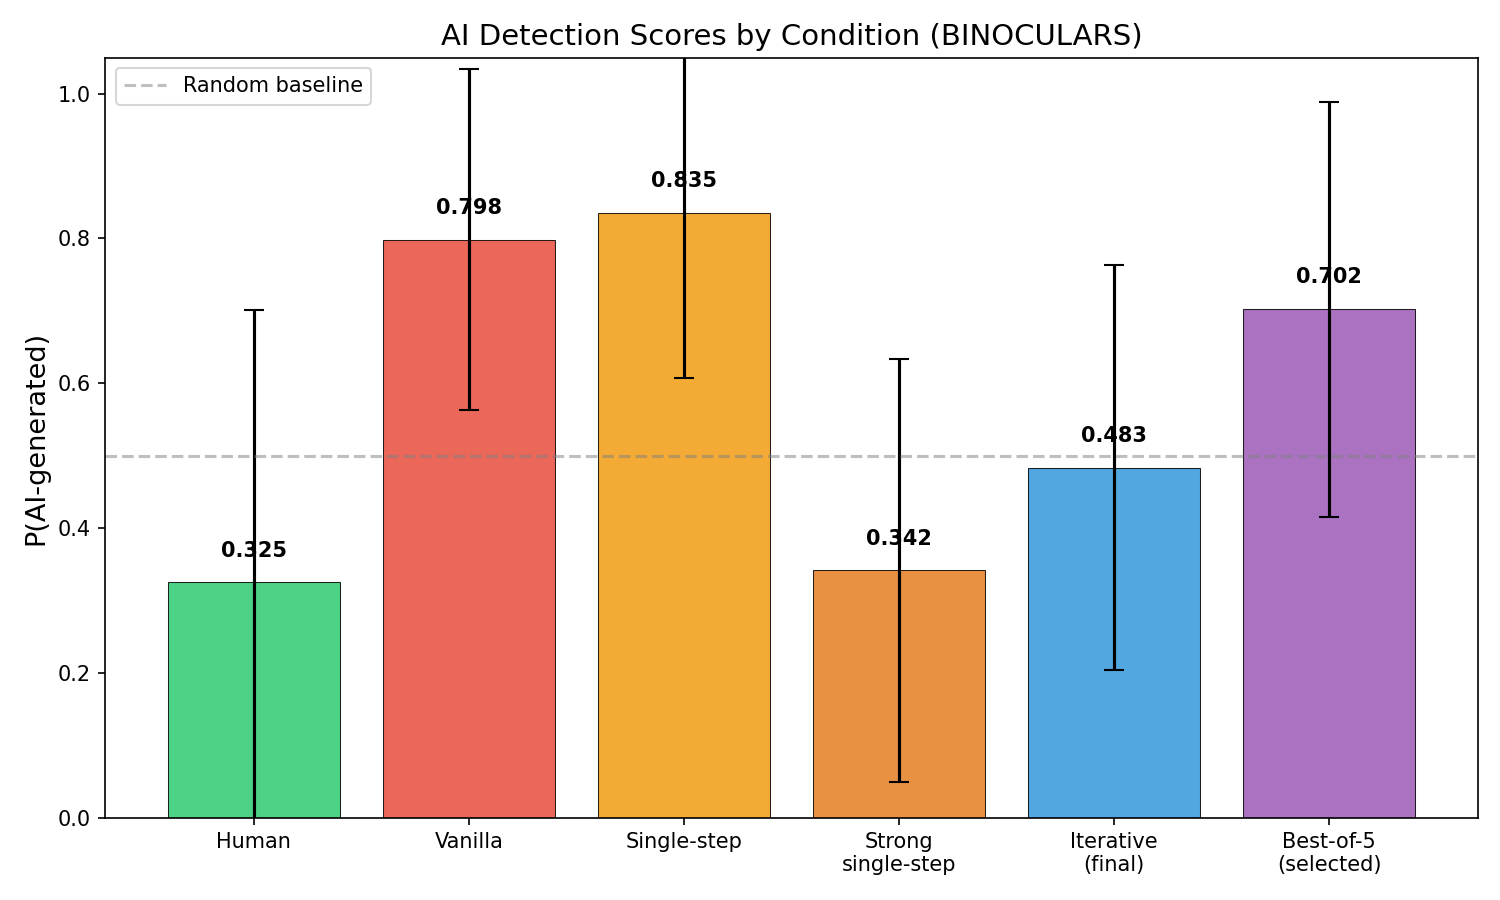
\includegraphics[width=0.95\linewidth]{figures/condition_comparison_binoculars.png}
\caption{Distribution of \binoculars detection scores across conditions. The strong single-step prompt and iterative rejection (R5) both shift the distribution toward human-level scores, while the naive single-step prompt remains close to vanilla.}
\label{fig:condition_comparison}
\end{figure}

\subsection{Iteration Trajectory}
\label{sec:trajectory}

\Figref{fig:trajectory} shows the mean \binoculars score at each rejection round. The trajectory is non-monotonic, with the largest single drop occurring between rounds 2 and 3 ($-$0.203), followed by a partial rebound at round 4.

\begin{figure}[t]
\centering
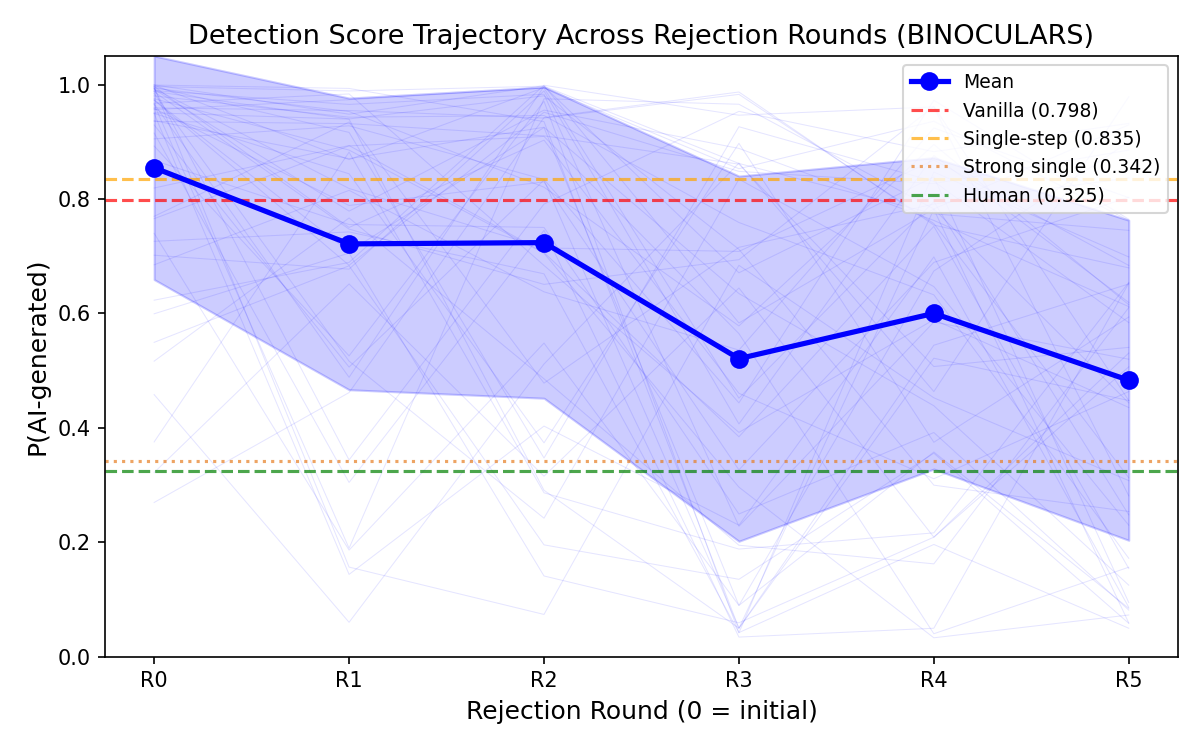
\includegraphics[width=0.95\linewidth]{figures/iteration_trajectory_binoculars.png}
\caption{Mean \binoculars $P(\text{AI})$ across rejection rounds. The sharpest improvement occurs between R2 and R3, suggesting a phase transition rather than gradual convergence. The non-monotonic pattern (R4 $>$ R3) indicates the model oscillates between generation regimes.}
\label{fig:trajectory}
\end{figure}

\tabref{tab:trajectory} reports the per-round scores. The overall trend is downward (R0: 0.855 $\to$ R5: 0.483), but the path is uneven. The R2$\to$R3 transition accounts for more than half of the total improvement, suggesting a tipping point in how the model responds to accumulated rejection context.

\begin{table}[t]
\centering
\caption{Per-round \binoculars scores during iterative rejection. The R2$\to$R3 transition shows the largest single-round improvement.}
\label{tab:trajectory}
\begin{tabular}{@{}lcc@{}}
\toprule
\textbf{Round} & \textbf{Mean $P(\text{AI})$} & \textbf{$\Delta$ from R0} \\
\midrule
R0 (initial) & 0.855 & --- \\
R1 & 0.722 & $-$0.133 \\
R2 & 0.724 & $-$0.131 \\
R3 & 0.521 & $-$0.334 \\
R4 & 0.600 & $-$0.255 \\
R5 (final) & 0.483 & $-$0.372 \\
\bottomrule
\end{tabular}
\end{table}

\subsection{Best-of-5 vs.\ Iterative Rejection}
\label{sec:bon}

A central question is whether iterative rejection provides genuine steering or merely benefits from selection pressure (\ie generating multiple outputs increases the chance of a low-scoring one). We control for this with the best-of-5 condition, which generates five independent vanilla outputs and selects the lowest-scoring one.

\tabref{tab:statistical} reports the statistical comparisons. Iterative rejection significantly outperforms best-of-5 selection on \binoculars (0.483 vs.\ 0.702, $p < 0.001$, $r = 0.555$), confirming that the rejection context provides steering beyond selection. The iterative approach achieves lower scores than best-of-5 on 36 of 50 questions (72\%).

\begin{table}[t]
\centering
\caption{Pairwise statistical comparisons against iterative rejection (R5) on \binoculars scores. All comparisons are significant after Bonferroni correction ($\alpha = 0.0125$). Effect sizes ($r$) are matched-pairs rank-biserial correlations.}
\label{tab:statistical}
\begin{tabular}{@{}lccc@{}}
\toprule
\textbf{Comparison} & \textbf{$p$-value} & \textbf{Effect size ($r$)} & \textbf{Significant} \\
\midrule
Single-step vs.\ Iterative & $1.08 \times 10^{-9}$ & 0.879 & Yes \\
Strong single-step vs.\ Iterative & $8.09 \times 10^{-3}$ & 0.426 & Yes \\
Best-of-5 vs.\ Iterative & $4.51 \times 10^{-4}$ & 0.555 & Yes \\
Vanilla vs.\ Iterative & $2.47 \times 10^{-7}$ & 0.776 & Yes \\
\bottomrule
\end{tabular}
\end{table}

\Figref{fig:bon_scatter} shows a per-question scatter plot comparing iterative rejection against best-of-5 selection. Most points fall below the diagonal, indicating iterative rejection achieves lower scores on the majority of questions.

\begin{figure}[t]
\centering
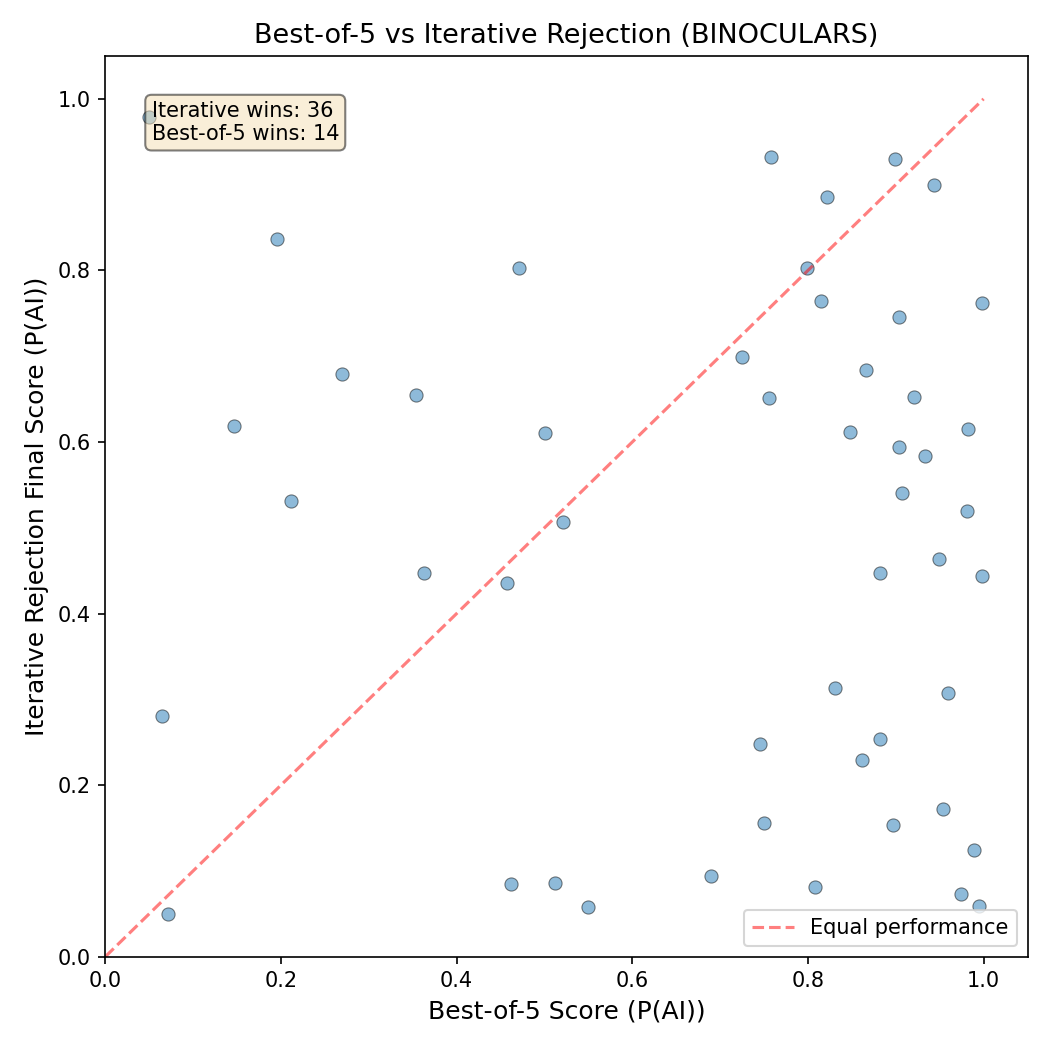
\includegraphics[width=0.7\linewidth]{figures/bon_vs_iterative_binoculars.png}
\caption{Per-question comparison of \binoculars scores: iterative rejection (R5) vs.\ best-of-5 selection. Points below the diagonal indicate questions where iterative rejection achieves lower (better) scores. The iterative approach wins on 72\% of questions.}
\label{fig:bon_scatter}
\end{figure}

\subsection{Linguistic Feature Analysis}
\label{sec:linguistic}

To understand \emph{how} the model changes its generation across rejection rounds, we track five linguistic features. \tabref{tab:linguistic} reports the values at the initial round (R0), final round (R5), and for human text.

\begin{table}[t]
\centering
\caption{Linguistic features across rejection rounds (\binoculars). The model increases vocabulary diversity and first-person pronoun usage (overshooting human norms) while failing to reduce AI marker words or increase contractions.}
\label{tab:linguistic}
\begin{tabular}{@{}lcccc@{}}
\toprule
\textbf{Feature} & \textbf{R0} & \textbf{R5} & \textbf{Human} & \textbf{Trend} \\
\midrule
Type-token ratio & 0.668 & 0.749 & 0.826 & \increase~toward human \\
First-person rate & 0.0006 & 0.016 & 0.002 & \increase\increase~overshoots \\
Contraction rate & 0.004 & 0.0004 & 0.005 & \decrease~away from human \\
AI marker count & 0.24 & 0.24 & 0.02 & $\rightarrow$ no change \\
Avg.\ sentence length & 20.0 & 19.3 & 21.8 & $\rightarrow$ minimal change \\
\bottomrule
\end{tabular}
\end{table}

\Figref{fig:linguistic} visualizes the per-round trajectories. Two patterns are noteworthy. First, the type-token ratio increases monotonically toward human levels, indicating richer vocabulary. Second, first-person pronoun usage increases 26$\times$ by R5, dramatically overshooting the human baseline (0.016 vs.\ 0.002). The model does not simply converge toward human statistics; it enters an exaggerated ``casual first-person'' mode.

Critically, the features the model \emph{fails} to change are equally informative. AI marker words (``delve,'' ``crucial,'' ``landscape'') remain at 0.24 per text, twelve times the human rate. Contraction rates actually decrease, contradicting the intuition that contractions sound more human. These failures suggest the model does not have fine-grained control over individual stylistic markers through rejection feedback alone.

\begin{figure}[t]
\centering
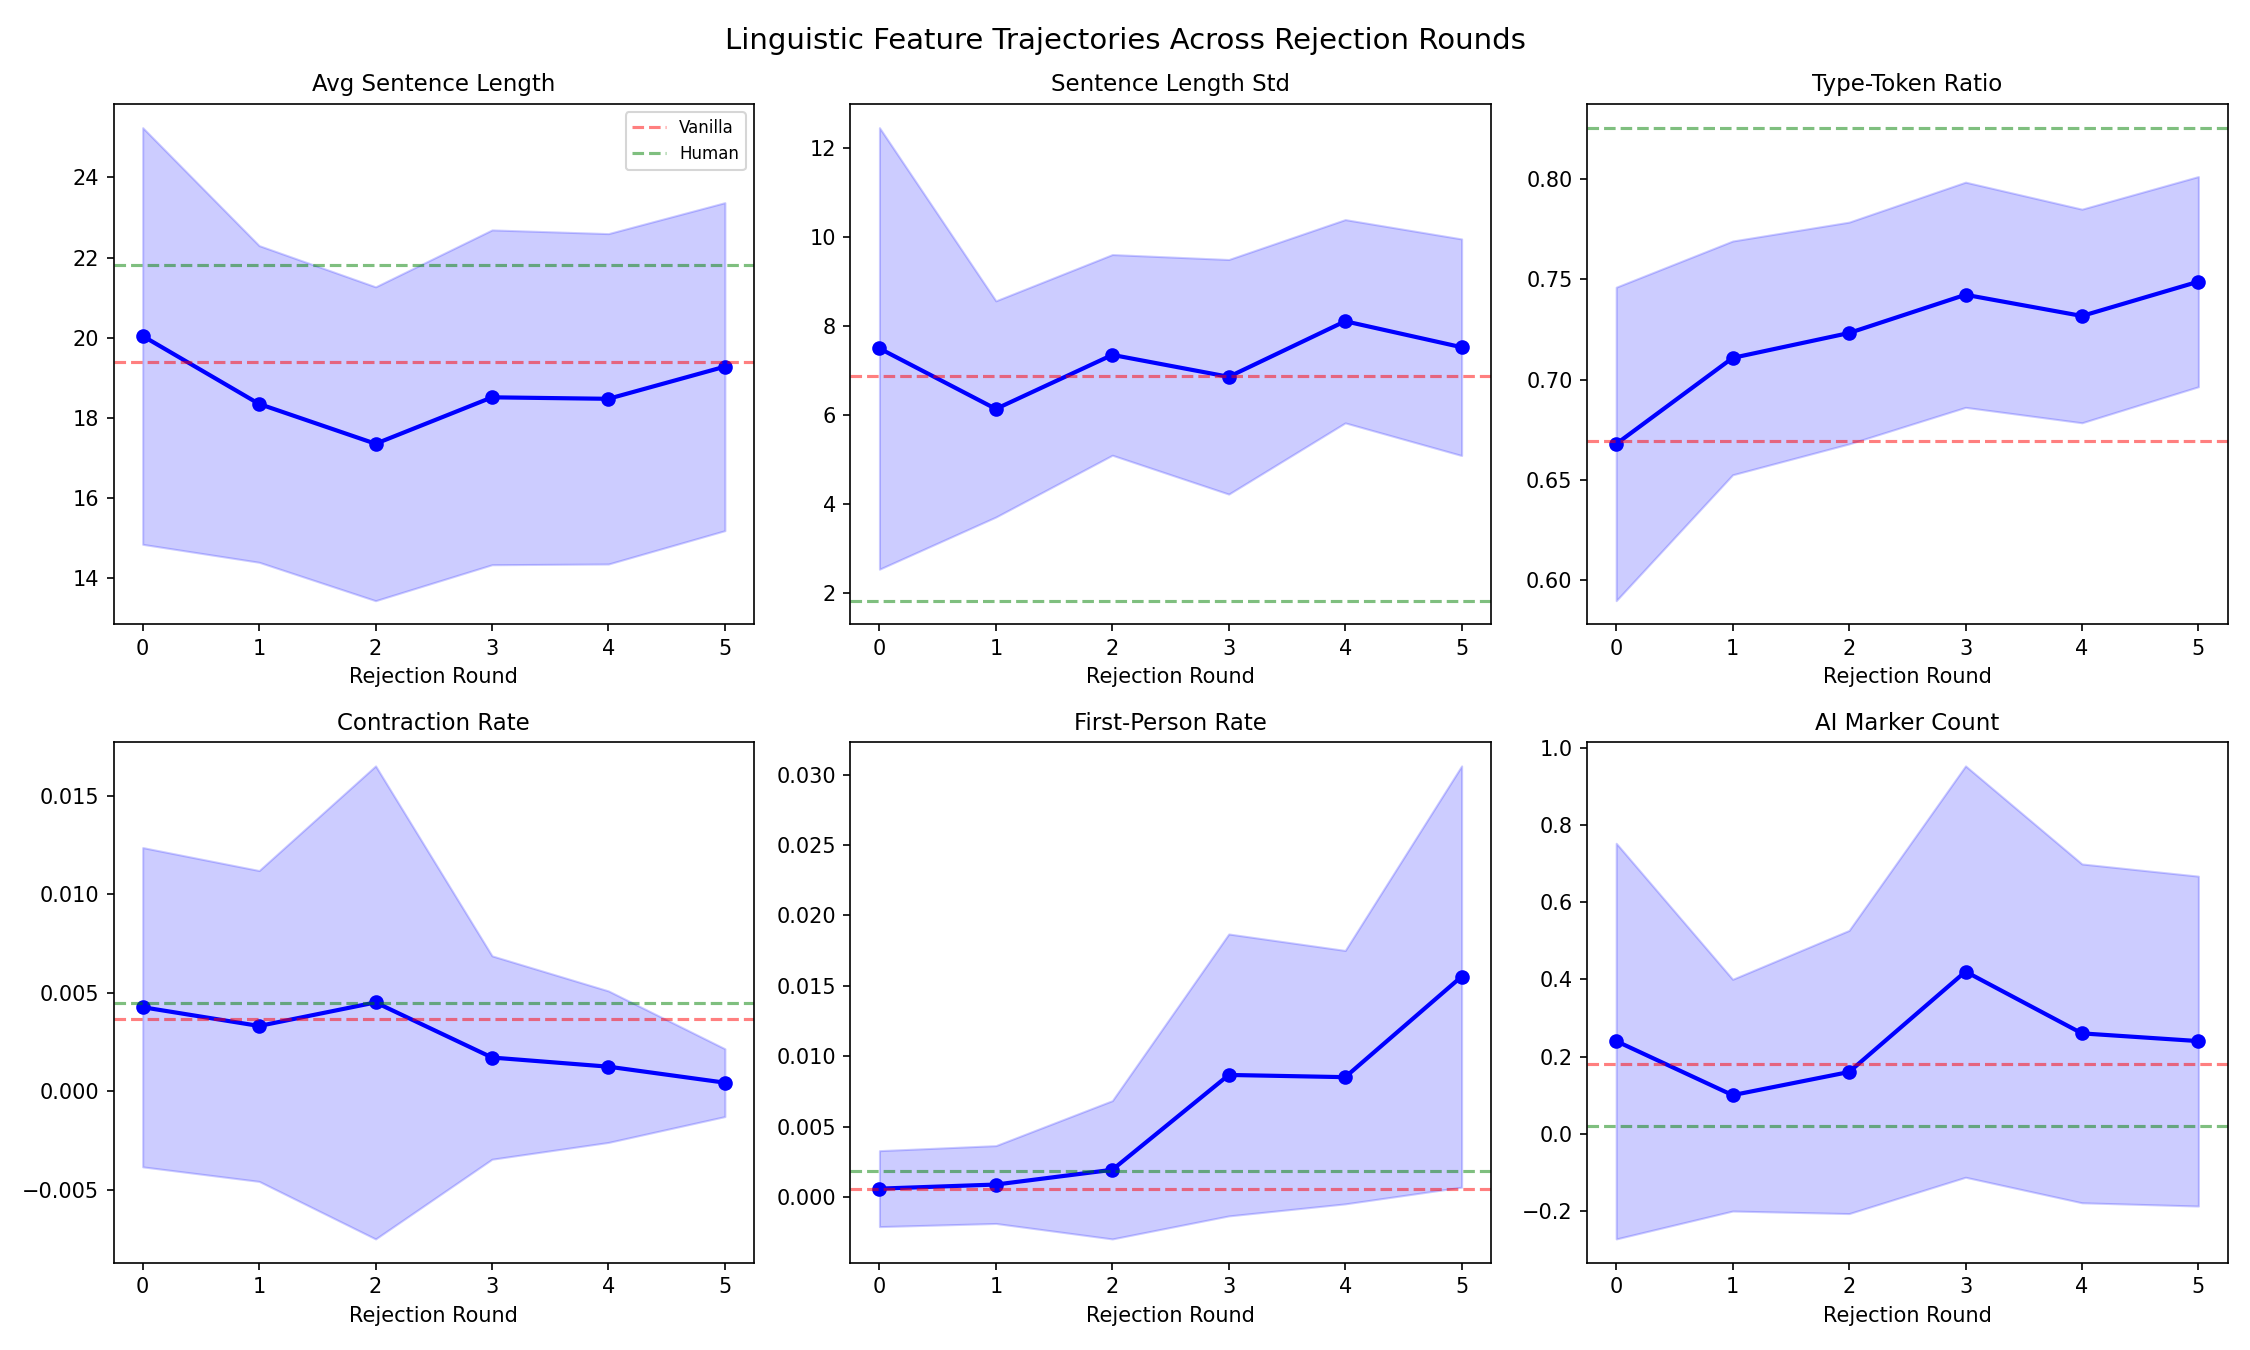
\includegraphics[width=0.95\linewidth]{figures/linguistic_features.png}
\caption{Linguistic feature trajectories across rejection rounds. Type-token ratio converges toward human levels, while first-person pronoun usage overshoots dramatically. AI marker words and contraction rates remain largely unchanged, indicating a regime shift rather than targeted feature suppression.}
\label{fig:linguistic}
\end{figure}
